\documentclass[12pt, a4paper]{article}
\usepackage[labelfont=bf]{caption}
\usepackage{diagbox}
\usepackage{fancyhdr}
\usepackage{float}
\usepackage[top=30mm, right=25mm, bottom=25mm, left=25mm]{geometry}
\usepackage{multicol}
\usepackage{parskip}
\usepackage{pgfplots}

\pagestyle{fancy}
\fancyhead[L]{COM3110}
\fancyhead[C]{Assignment: Document Retrieval}
\fancyhead[R]{Zer Jun Eng}

\pgfplotsset{width=10cm,compat=1.9}

\begin{document}

\section{Implementation of Weighting Scheme}
Before implementing the weighting schemes, it is necessary to create a list of candidate documents
for each query to improve the retrieval efficiency. Candidate documents are those that contains at
least one `term' from the query. Hence the list of candidate documents can be generated using list
comprehension with sets intersection function. In addition, when calculating the size of each
document vector, it is only required to loop through all the `term' that is in the document, thus
saving a lot of computational cost.

All term weighting schemes are implemented using vector space model, which is represented as the
modified equation with the component $\sqrt{\sum\nolimits_{i=1}^n q_i^2} $ dropped:

\begin{center}
  $ SIM(Q, D) = \frac{\sum\nolimits_{i=1}^n q_i d_i}{\sqrt{\sum\nolimits_{i=1}^n d_i^2}}$
\end{center}

% $\sum\nolimits_{i=1}^n q_i d_i$ $\sqrt{\sum\nolimits_{i=1}^n d_i^2}$.

\subsection{Binary}
The term weight is either 1 or 0. $q_i d_i$ increases by 1 if the term is in the query, and $d_i^2$
increases by 1 if the term is in the document. The similarity score of a document is higher if it
contains more terms from the query.

\subsection{Term Frequency}
The term weight is equal to the term frequency in a specific document and the query. The similarity
score of a document is higher if it contains more terms that have higher frequency the document and
the query.

\subsection{Term Frequency - Inverse Document Frequency (TFIDF)}
The TFIDF scheme is fully implemented. The term weight depends on its frequency in the relevant
documents, query, and in the collection.

\section{Results}
\begin{multicols}{2}
  \def\arraystretch{1.2}
  \textbf{No} stoplist, \textbf{No} stemming
  \begin{table}[H]
    \begin{tabular}{|c||c||c||c|}
    \hline
              & Binary & TF   & TFIDF \\ \hline
    Rel\_Retr & 44     & 50   & 132   \\ \hline
    Precision & 0.07   & 0.08 & 0.21  \\ \hline
    Recall    & 0.06   & 0.06 & 0.17  \\ \hline
    F-measure & 0.06   & 0.07 & 0.18  \\ \hline
    \end{tabular}
  \end{table}

  \columnbreak

  \textbf{No} stoplist, \textbf{With} stemming
  \begin{table}[H]
    \begin{tabular}{|c||c||c||c|}
    \hline
              & Binary & TF   & TFIDF \\ \hline
    Rel\_Retr & 59     & 73   & 166   \\ \hline
    Precision & 0.09   & 0.11 & 0.26  \\ \hline
    Recall    & 0.07   & 0.09 & 0.21  \\ \hline
    F-measure & 0.08   & 0.10 & 0.23  \\ \hline
    \end{tabular}
  \end{table}
\end{multicols}
\pagebreak
\begin{multicols}{2}
  \textbf{With} stoplist, \textbf{No} stemming
  \begin{table}[H]
    \begin{tabular}{|c||c||c||c|}
    \hline
              & Binary & TF   & TFIDF \\ \hline
    Rel\_Retr & 81     & 103  & 140   \\ \hline
    Precision & 0.13   & 0.16 & 0.22  \\ \hline
    Recall    & 0.10   & 0.13 & 0.18  \\ \hline
    F-measure & 0.11   & 0.14 & 0.19  \\ \hline
    \end{tabular}
  \end{table}

  \columnbreak

  \textbf{With} stoplist, \textbf{With} stemming
  \begin{table}[H]
    \begin{tabular}{|c||c||c||c|}
    \hline
              & Binary & TF   & TFIDF \\ \hline
    Rel\_Retr & 105    & 126  & 172   \\ \hline
    Precision & 0.16   & 0.20 & 0.27  \\ \hline
    Recall    & 0.13   & 0.16 & 0.22  \\ \hline
    F-measure & 0.15   & 0.18 & 0.24  \\ \hline
    \end{tabular}
  \end{table}
\end{multicols}

\begin{figure}[H]
  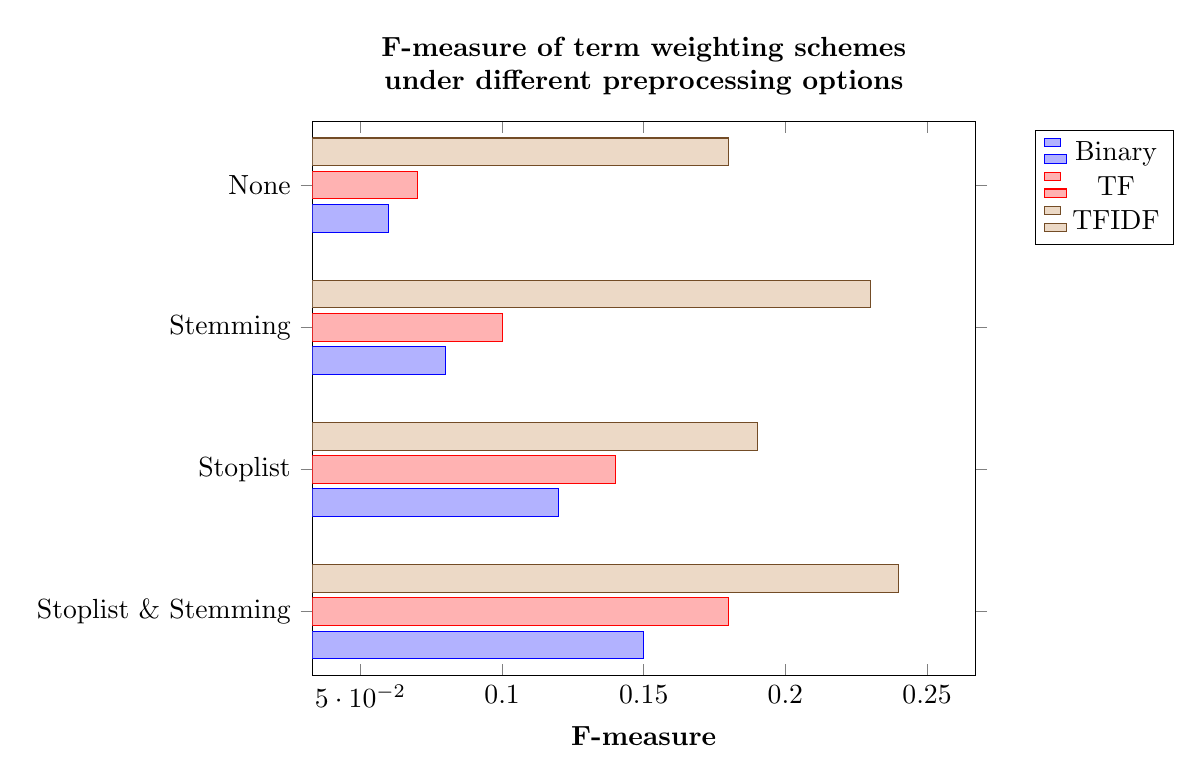
\begin{tikzpicture}
    \begin{axis}[
        xbar,
        enlargelimits=0.15,
        legend style={at={(1.3,0.88)},anchor=east,legend columns=1},
        xlabel={\textbf{F-measure}},
        title style={align=center},
        title={\textbf{F-measure of term weighting schemes} \\ \textbf{under different preprocessing options}},
        symbolic y coords={Stoplist \& Stemming,Stoplist,Stemming,None},
        ytick=data
        ]
      \addplot coordinates {(0.15,Stoplist \& Stemming) (0.12,Stoplist) (0.08,Stemming) (0.06,None)};
      \addplot coordinates {(0.18,Stoplist \& Stemming) (0.14,Stoplist) (0.10,Stemming) (0.07,None)};
      \addplot coordinates {(0.24,Stoplist \& Stemming) (0.19,Stoplist) (0.23,Stemming) (0.18,None)};
      \legend{Binary, TF, TFIDF}
    \end{axis}
  \end{tikzpicture}
  \captionof{figure}{F-measure bar chart of three term weighting schemes}
\end{figure}


\section{Discussion and Conclusion}
% Is the report a clear and accurate description of the implementation? How complete and accurate is
% the discussion of the performance of the system under a range of configurations? What inferences
% can be drawn about the performance of the IR system from these results?

\end{document}
